\documentclass[a4paper,11pt]{article}

% Identificação
\newcommand{\rtmodulo}{III}
\newcommand{\rttitulo}{Game Design Document - GDD}
\newcommand{\rtdisciplina}{Projeto Integrador}
\newcommand{\rttituloprof}{Professor formador}
\newcommand{\rtprofessor}{Suâmi Abdalla-Santos}

\usepackage{sty/ifb}
\usepackage{wrapfig} % Imagens que se cruzam com texto

%----------------------------------------------------------------------
% Início do Documento
%-----------------------------------------------------------------------
\begin{document}

\title{\rttitulo}
\author{Fernando Antonio Fernandes Anselmo} 
\date{Junho de 2019}

\begin{titlepage}
	\centering
	\vspace*{0.5 cm}
	
\includegraphics[scale = 0.65]{imagens/logo.png}\\[1.0 cm]
	\textsc{\Large Instituto Federal de Brasília}\\[2.0 cm]
	\textsc{\Large Técnico em Programação de Jogos Digitais \\ Módulo \rtmodulo}
	\rule{\linewidth}{0.2 mm} \\[0.4 cm]
	{ \huge \bfseries \rttitulo}\\
	\rule{\linewidth}{0.2 mm} \\[1.5 cm]
	\begin{minipage}{1.0\textwidth}
		Disciplina: \rtdisciplina \\  
		\rttituloprof: \rtprofessor \\
		Aluno: Fernando Antonio Fernandes Anselmo \\
		Turma: Turma A \\
		Polo: Brasília
	\end{minipage}\\[2 cm] 
\end{titlepage}



% Corpo do Documento
\section{Histórico}
"\textbf{Missile Command}" foi um dos primeiros jogos da Atari a se tornar bastante popular entre os jogadores de vídeo game de sua época, em grande parte devido à proposta interessante de jogo, que era proteger uma cidade, com uma bateria anti-aérea fixa, do ataque de mísseis vindos do céu.

"\textbf{Defender}" foi outro jogo de lançado para o Atari. Nele o jogador controlava uma nave armada de raios laser, e a sua missão era defender uma grande cidade do ataque de alienígenas. O jogo possuía dezenas de fases com grau de dificuldade crescente. Ambos jogos podem provavelmente serem considerados como jogos infinitos.

\section{Resumo}
"\textbf{Dragon Defender}" é um jogo no mesmo estilo dos jogos citados anteriormente, porém pode ser considerado como uma mistura de ambos. O objetivo é controlar um Dragão de Gelo que está ameaçado de morte por mísseis vindo do espaço e deve usar seu raio para destruí-los.

Diferente do jogo original (\textit{Missile Command}) que era uma torre parada que atirava em ângulos, o dragão pode se movimentar (como em \textit{Defender}) por todas as direções lançando seus raios para deter os mísseis impedindo-os de cair em seu lar. Porém não pode tocá-los pois eles explodem, causando-lhe um dano maior.

\section{Gameplay}
\textbf{Drogo} é um Dragão Azul que acaba de acordar nas gélidas terras do ártico e lá descobriu que está intimamente ligado ao seu lar. A humanidade tem um pavor inexplicado de Dragões e não quer nem conversa, resolveu enviar seu arsenal de mísseis para destruir o lar de Drogo e assim acabar de uma vez por todas com o Dragão.

\section{Ambiente do Jogo}
Por ser um dragão de gelo obviamente o cenário deve ser do ártico, uma característica de todo o jogo é que tanto o cenário quanto Drogo possuem a cor predominantemente "Azul".

\begin{figure}[!htb]
	\centering
	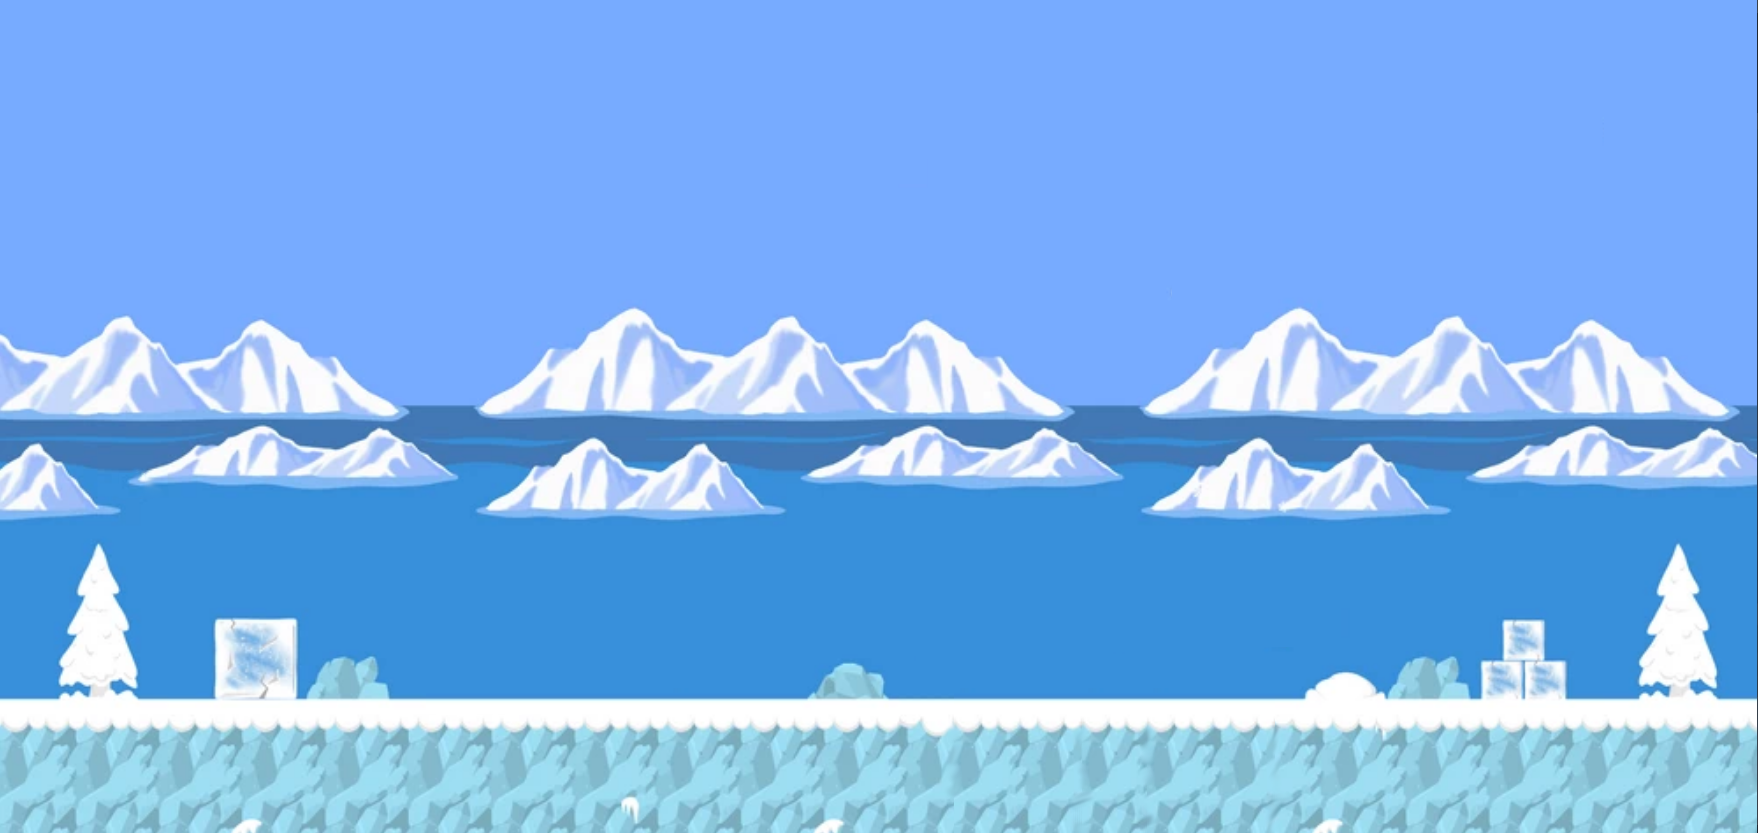
\includegraphics[width=0.83\textwidth]{imagens/pi-Fundo.png}
	\caption{Cenário de Fundo}
\end{figure}

O background é formado pelo cenário por uma paisagem do ártico que reflete o lar de Drogo no qual os mísseis irão tentar destruí-lo.

\subsection{Personagens}
"Drogo" como dito é um dragão de gelo, sendo assim possui a cor predominantemente azul.
\begin{figure}[!htb]
	\centering
	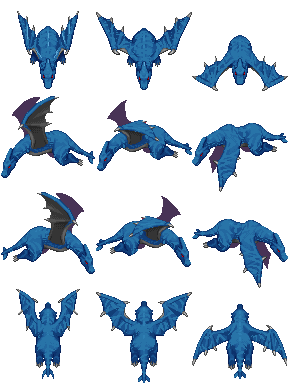
\includegraphics[width=0.6\textwidth]{imagens/pi-DragaoDef.png}
	\caption{Sprite para Drogo}
\end{figure}

Os mísseis estão na cor entre o "Amarelo" (menor dano) e o "Vermelho" (maior dano).
\begin{figure}[!htb]
	\centering
	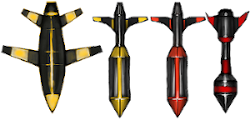
\includegraphics[width=0.4\textwidth]{imagens/pi-Misseis.png}
	\caption{Mísseis em ordem de dano crescente}
\end{figure}

Observamos que contrastando a tudo os mísseis (que são os vilões da história) estão em uma cor totalmente oposta a todo o ambiente do jogo.

\section{Mecânicas}
Cada um dos tipos de mísseis causa um determinado dano em Drogo e no que ele conhece por lar, podendo chegar a matá-lo. Os danos causados por cada um dos mísseis são diferentes, tanto se "Drogo" encostar nele quando se cair em seu lar, conforme a seguinte tabela:

\textbf{Míssel modelo Z480-56}

\begin{minipage}{\textwidth}
	\begin{wrapfigure}{l}{0.10\textwidth}
		\vspace{-\baselineskip}
		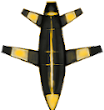
\includegraphics[width=0.8\linewidth]{imagens/pi-Misseis1.png} 
	\end{wrapfigure}
	Esse é um míssel no estilo Drone que pode possui boa velocidade. Causa um dano de 1\% de vida se atinge o solo e 5\% se Drogo encostar nele e o mesmo explodir. Um simples raio de "Drogo" o destrói. Possui o valor de 1 ponto para o jogador.
	\vspace{10pt}
\end{minipage}

\textbf{Míssel modelo Z480-786}

\begin{minipage}{\textwidth}
	\begin{wrapfigure}{l}{0.10\textwidth}
		\vspace{-\baselineskip}
		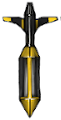
\includegraphics[width=0.6\linewidth]{imagens/pi-Misseis2.png} 
	\end{wrapfigure}
	Esse é um míssel armado com uma primitiva ogiva um pouco mais lento. Causa um dano de 5\% de vida se atinge o solo e 10\% se Drogo encostar nele e o mesmo explodir. É destruído com 2 raios de "Drogo". Possui o valor de 2 pontos para o jogador.
	\vspace{30pt}
\end{minipage}
	
\textbf{Míssel modelo Z480-786 II}

\begin{minipage}{\textwidth}
	\begin{wrapfigure}{l}{0.10\textwidth}
		\vspace{-\baselineskip}
		
\includegraphics[width=0.6\linewidth]{imagens/pi-Misseis3.png} 
	\end{wrapfigure}
	Esse é um míssel armado com uma ogiva térmica é lento. Causa um dano de 10\% de vida se atinge o solo e 20\% se Drogo encostar nele e o mesmo explodir. É destruído com 2 raios de "Drogo".  Possui o valor de 2 pontos para o jogador.
	\vspace{30pt}
\end{minipage}

\textbf{Míssel modelo Z480-Zilog}

\begin{minipage}{\textwidth}
	\vspace{5pt}
	\begin{wrapfigure}{l}{0.10\textwidth}
		\vspace{-\baselineskip}
		
\includegraphics[width=0.5\linewidth]{imagens/pi-Misseis4.png} 
	\end{wrapfigure}
	Esse é um míssel armado com uma ogiva térmica do tipo Nuclear é bem lento. Causa um dano de 25\% de vida se atinge o solo e 50\% se Drogo encostar nele e o mesmo explodir. É destruído com 3 raios de "Drogo". Possui o valor de 3 pontos para o jogador.
	\vspace{20pt}
\end{minipage}

"Drogo" consegue lançar raios de gelo que destroem os mísseis conforme indicado para cada modelo. Os mísseis parcialmente destruídos não perdem seu poder. Assim como \textit{Missile Command} vários deles cairão simultaneamente e cabe ao jogador destruir o máximo que conseguir ou tomar a decisão de qual destruir para evitar um maior dano.

Um detalhe interessante é que o jogo pode ser considerado como jogabilidade infinita, e assim como seus antecessores não existe uma missão completa apenas um aumento de dificuldade a medida que o tempo vai avançando. Sendo assim é interessante marcar o maior placar de pontuação atingida.

\end{document}
